\documentclass[../notes.tex]{subfiles}

\graphicspath{{\subfix{../img/}}}

\begin{document}

\section{CSC473: Advanced Algorithms}

\subsection{Global Min-Cut}


\textbf{Given} an undirected, unweighted, and connected graph $ G = (V, E) $, \textbf{return} the smallest set of edges that disconnects $ G $



\begin{figure}[H]
  \centering
  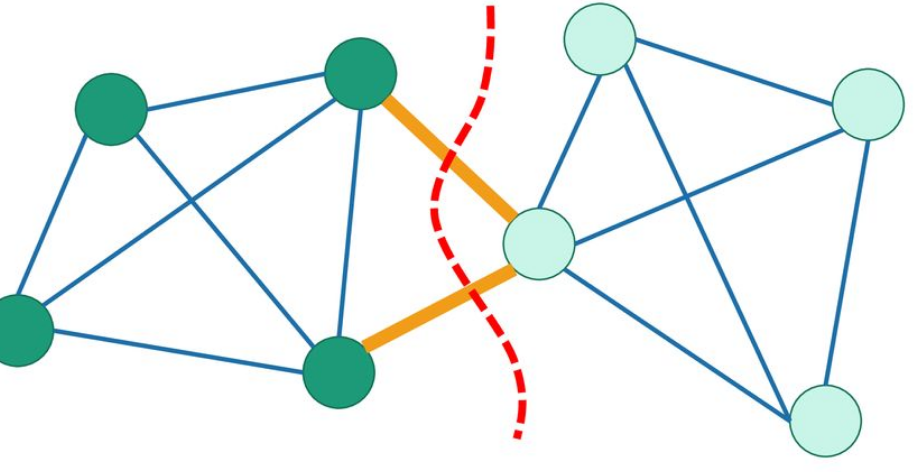
\includegraphics[width=0.8\linewidth]{img/image_2023-01-09-12-40-24.png}
  \caption{Example of global min-cut. Note that the global min-cut is not necessarily unique}
\end{figure}

\marginnote{An example of where this may be useful is in computer networks where we can measure the resiliency of a network by how many cuts must be made before a vertex (or many) get disconnected}


\begin{lemma}
  If the min cut is of size $ \ge k $, then $ G $ is $ k $-edge-connected
\end{lemma}

It may be more convenient to return a set of vertices instead

\begin{definition}
  
\begin{equation}
  S, T \subseteq V, S \cap T = \varnothing 
\end{equation}

\begin{equation}
  E(S,T) = \{(u,v) \in E : u \in S, v \in T\} 
\end{equation}

The global min-cut is to output $ S \subseteq V $ such that $ S \neq \varnothing, S \neq V $,  such that $ E(S, V\setminus S ) $ is minimized.


\end{definition}

\begin{blockquote}

Note that the min-cut-max-flow problem is somewhat of a dual to the global min-cut problem; the min-cut-max-flow problem imposes a few more constraints than the global min-cut algorithm i.e. having a directed and weighted graph as well as the notion of a source or sink.

\begin{itemize}
  \item \textbf{Input: }  Directed, weighted, and connected $ G = (V,E) $, $ s \in V, t \in V $
  \item \textbf{Output}  : $ S $ such that $ s \in S, t \notin S $ such that $  |E(S, V\setminus S ) |  $ is minimized
\end{itemize}
  
\end{blockquote}

We can kind of intuitively see that the global min-cut can be taken to the minimum of all max-flows across the graph.
So we can take the max-flow solution and then reduce it to find the global min cut.

Question: how many times will we have to run max-flow to solve the global min-cut problem? 
Naively, we may fix $ t $ to be an arbitrary node, then try every other $ s \neq t $ to find the $  s-t $ min-cut to get the best global min-cut.

We know from previous courses that the Edmonds-Karp max-flow algorithm will run in $ O(nm^2) = O(n^5) $, which makes our global min-cut algorithm $ O(n^6) $.
However, there is a paper recently published which gives an algorithm for min-cut in nearly linear time, i.e $ O(m^{1-O(1)}) = O(n^2) $  which gives a global min-cut runtime of $ O(n^3) $.

A randomized algorithm will be presented that solves this problem in $ O(n^2 \log^2 n) $



















\end{document}
